% Test tex file!

\documentclass[a4paper,12pt]{article}
\usepackage{times}  % DO NOT CHANGE THIS
\usepackage{helvet} % DO NOT CHANGE THIS
\usepackage{courier}  % DO NOT CHANGE THIS
\usepackage[hyphens]{url}  % DO NOT CHANGE THIS
\usepackage{graphicx} % DO NOT CHANGE THIS
\urlstyle{rm} % DO NOT CHANGE THIS
\def\UrlFont{\rm}  % DO NOT CHANGE THIS
\usepackage{natbib}  % DO NOT CHANGE THIS AND DO NOT ADD ANY OPTIONS TO IT
\usepackage{caption} % DO NOT CHANGE THIS AND DO NOT ADD ANY OPTIONS TO IT
\frenchspacing  % DO NOT CHANGE THIS
\setlength{\pdfpagewidth}{8.5in}  % DO NOT CHANGE THIS
\setlength{\pdfpageheight}{11in}  % DO NOT CHANGE THIS
\usepackage{algorithm} %format of the algorithm 
\usepackage{algorithmic} %format of the algorithm 
\usepackage{multirow} %multirow for format of table 
\usepackage{amsmath} 
\usepackage{xcolor}
\usepackage{amssymb}
\usepackage{amsmath}
\usepackage{CJKutf8}
\usepackage{courier}


\begin{CJK}{UTF8}{gbsn}
% \begin{CJK}{UTF8}{gkai}
\begin{document}
\title{强化学习：作业一}

\author{杨皓天 502023370059}

\date{2023-10-13}

\maketitle

\section{作业内容}
\noindent在“蒙特祖马的复仇”环境中实现Dagger算法。

\section{实现过程}

\quad\quad首先安装环境依赖，安装了gym和附属插件保证程序能够运行蒙特祖马的复仇，我使用的库版本为：gym=0.26.2，ale-py=0.8.1，matplotlib=3.7.1,  python=3.8并且对gym使用accept-rom-licence操作，成功运行了蒙特祖马的复仇游戏。

之后我在Dagger.py里采用了CNN模型，并在MyDagger类中进行了调用，并实现其中的模型训练（update），以及测试时的动作选择（select\_action），由于CNN计算消耗较大，我对agent更新次数和训练轮数以及相应的测试参数进行了调整。

然后在运行main之后的数据标注过程中，我发现原始代码每次运行会覆盖标记过的图片，于是将save\_img参数改为了false，并将数据标注的过程移动到play game环节，使用matplotlib中的库函数实现了交互式数据标注。本次实验专家数据采用的策略是：先在第一个房间拿到钥匙，得到100分，之后打开右边的门，得到400分，然后躲过幽灵向下走楼梯，拿到武器，得到500分，最后上楼梯返回，击杀一个幽灵，得到2500分。由于样本数量的原因，在训练时采用了每进行一次agent update，训练数据集增加400条专家序列的方式。

\section{复现方式}
\noindent在主文件夹下运行 \texttt{python main.py}.
\section{实验效果}
\noindent见图 \ref{performance}。其中每进行一次update，agent就会进行4轮训练并更新参数。多次访问专家数据后，agent就会进行两次进行600步动作的测试（这里对参数进行了调整），获取done时的reward，最终呈现的实验结果如图所示。其中，我发现，随着访问次数的增加和训练轮数的迭代，agent能够得到的奖赏在逐步增加，最终逼近专家的行动策略。
\begin{figure}[h!]
\centering
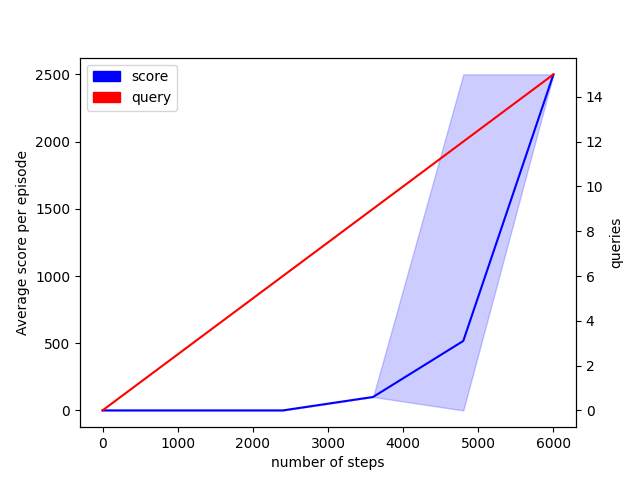
\includegraphics[width=8cm,height=7cm]{code/performance.png}
\caption{Dagger算法}
\label{performance}
\end{figure}
\section{小结}
\quad\quad在这次实验中，我发现Dagger算法需要多次访问专家，agent的表现与数据集的质量以及专家策略具有很强的相关性，需要花费大量精力进行数据标注，agent训练时也会出现不稳定性，3000多步的时候才能稳定的拿到钥匙，最终在增加数据量和训练轮数的情况下，才能逼近专家策略。另外，Dagger算法并不稳定，在整体的实验过程中，我进行了多次重复实验，报告里展示了效果最佳的一次。由此可见，该算法训练成本非常高，适用场景也很有限，并且随着样本数量的增加，模型训练时间和占用的计算资源也在逐渐增加，回报很低，对此我们需要更加高效的算法。


\end{document}

\end{CJK}